\chapter{Method}
For our experiments, we follow the steps depicted in Figure \ref{fig:pipeline}.
\begin{figure}[ht]
    \centering
    
\includegraphics[width=1.0\linewidth]{img/pipeline.png}
    % \includesvg[pretex=\tiny, width=1.0\linewidth]{img/pipeline}
    \caption{Visualization of our pipeline for \ac{lod} generation. Yellow files that are an input or output to green program components.}
    \label{fig:pipeline}
\end{figure}
We first take the surface meshes and apply the filtering procedure to obtain the volume grids.
Additionally we save metadata like the bounding-box sizes of the grids, which we then need for scene generation.
This generation step can either generate ground-truth scenes that only contain meshes or it can generate scenes that use \acp{lod}.
The next step in the pipeline is the rendering of the scene, which uses mesh or volume files depending on the definitions in the generated scene file.
Finally we evaluate our results by comparing the mesh-only renderings with the ones that use \ac{lod}.

Our surface models are free tree meshes from XfrogPlants \cite{xfrogplants} and the McGuire Computer Graphics Archive \cite{McGuire2017Data}.

\section{Mesh filtering}
\label{sec:mesh_filtering}
As described in Section \ref{sec:transforming_meshes_into_volumes} we use the ray casting approach by \citeauthor{hybrid_mesh_volume_lods} with a few modifications for our filtering \cite{hybrid_mesh_volume_lods}.
The ray casting is \ac{gpu} accelerated using OptiX \cite{parker_optix}.
In contrast to \citeauthor{hybrid_mesh_volume_lods} we assume our particles to have an isotropic microflake projected area $\sigma$, meaning that it is not view dependent.
This simplifies our optimization procedure for now, but we can still extend the procedure for anisotropic particles later.
The origin of our rays are uniformly sampled in each voxel and the direction is uniformly sampled over the hemisphere.
\citeauthor{hybrid_mesh_volume_lods} use a ray length that is equal to the edge length of a voxel, which leads to a blurring since adjacent geometry is included in the density estimation.
As \citeauthor{wang_object_space_aliasing} points out, this can reduce object space aliasing \cite{wang_object_space_aliasing}.
However we think, that we can increase the spatial resolution while preserving the blurring by clipping the ray at a bounding sphere.
We position the sphere at the voxel's center and scale it so that its diameter is slightly larger than the diagonal of the voxel.
Each ray is then first intersected with this sphere to compute a $t_{max}$, before the intersection test with the mesh geometry happens.
Figure \ref{fig:raygen_filtering} compares our approach for determining the ray length with the approach of \citeauthor{hybrid_mesh_volume_lods}.
\begin{figure}[ht]
    \centering
    \begin{subfigure}[b]{0.25\linewidth}
        \centering
        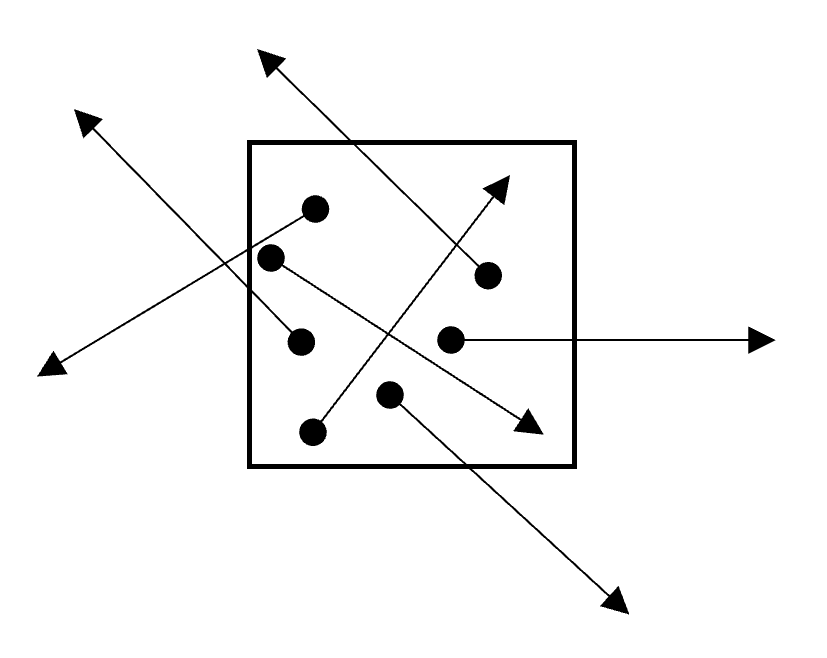
\includegraphics[width=\linewidth]{img/raygen_filtering_unclipped.png}
        \caption{}
        \label{fig:raygen_filtering_unclipped}
    \end{subfigure}
    \begin{subfigure}[b]{0.25\linewidth}
        \centering
        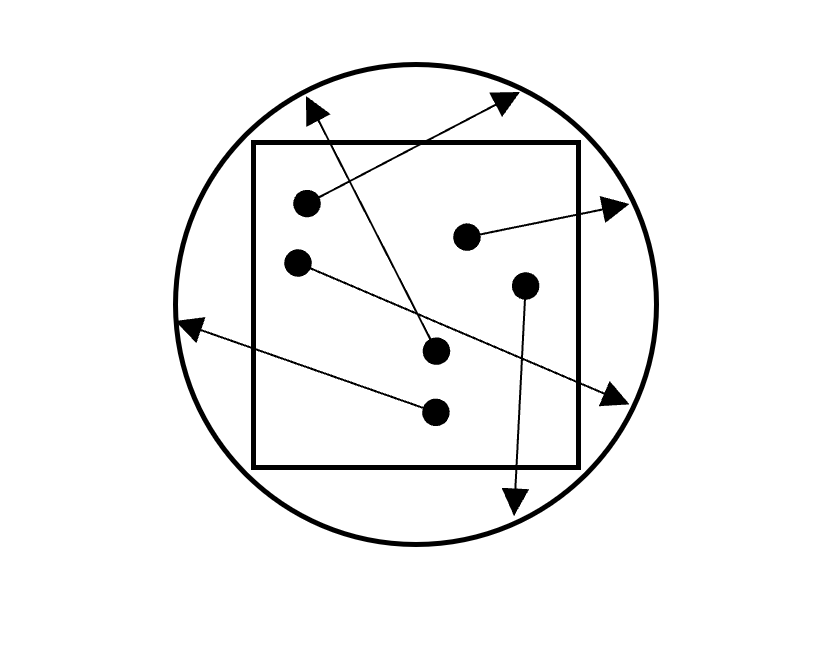
\includegraphics[width=1\linewidth]{img/raygen_filtering_clipped.png}
        \caption{}
        \label{fig:raygen_filtering_clipped}
    \end{subfigure}
	\caption{Image (a) shows the approach by \citeauthor{hybrid_mesh_volume_lods} with constant ray length. Figure (b) shows our approach with ray clipping at a bounding sphere.}
	\label{fig:raygen_filtering}
\end{figure}

With these modifications we also have to solve a different integral than that from Equation \ref{eq:loubet_filtering_equation}.
We therefore have to find a density $\rho$ that suffices:
\begin{equation}
    1 - \frac{1}{4\pi}\int_{\mathcal{S}^2} e^{-\rho\sigma ray_l(\omega)} d\omega = P_{occ}.
    \label{eq:our_filtering_equation}
\end{equation}
Note that the projected area $\sigma$ is now independent of the direction $\omega$, whereas the ray length depends on $\omega$, since the rays are clipped by the bounding sphere.
As stated in Section \ref{sec:transforming_meshes_into_volumes}, we cannot solve for the density with analytical methods, therefore we iteratively optimize $rho$:
\begin{equation*}
    \rho_{i+1}=\rho_i - \alpha (P_{occ,volume} - P_{occ,mesh}),
\end{equation*}
where $i$ denotes the iteration, $\alpha$ is a learning rate, $P_{occ,mesh}$ is the ratio of geometry hits to the total number of rays casted and $P{occ,volume}$ is the probability that a medium interaction takes place given the density $\rho$.
It is computed by Monte Carlo integrating Equation \ref{eq:our_filtering_equation}, so our estimator has the form:
\begin{equation*}
    1 - \frac{1}{N}\sum_{n=1}^{N} e^{-\rho\sigma ray_l(\omega_n)} = P_{occ,volume}.
\end{equation*}
Apart from this density estimate we also filter the diffuse and specular color of the geometry, the normals, the index of refraction and the SGGX Matrix $S$ by averaging.
The Matrix $S$ serves later as a coordinate frame for sampling reflection directions with the phase function \cite{sggx}.

% In total our attributes occupy 80 bytes of memory per voxel and we first represent them by a dense grid in the \ac{GPU}'s global memory.
We represent these attributes as a dense grid in the \acs{gpu}'s global memory.
OpenVDB cannot be used for this, because we were not able to integrate it in the CUDA device code, NanoVDB on the other hand, is a read-only grid.
Only after copying the dense grid to host memory we convert it into an OpenVDB grid and subsequently into a NanoVDB grid which we store to disk.
Using NanoVDB however, imposes a limit of storing 32 bytes per voxel.
Because our attributes occupy 80 bytes of memory we use quantization to represent the values in the grid and before doing computations like interpolation or shading we transform them back to the full width.
The following table summarizes the size of all attributes in regular and quantized format (ignoring padding):
\begin{center}
    \begin{tabular}{| c | c | c | }
        \hline
         & Regular Format & Quantized Format \\
         \hline
         Density & $1\times 4\;\text{bytes}$ & $1\times 4\;\text{bytes}$ \\
         \hline
         $S$ & $9\times 4\;\text{bytes}$ & $6\times 2\;\text{bytes}$ \\
         \hline
         Diffuse color & $3\times 4\;\text{bytes}$ & $3\times 1\;\text{bytes}$ \\
         \hline
         Specular color & $3\times 4\;\text{bytes}$ & $3\times 1\;\text{bytes}$ \\
         \hline
         Normal & $3\times 4\;\text{bytes}$ & $3\times 2\;\text{bytes}$ \\
         \hline
         Index of refraction & $1\times 4\;\text{bytes}$ & $1\times 2\;\text{bytes}$ \\
         \thickhline
         Total & $80\;\text{bytes}$ & $30\;\text{bytes}$ \\
         \hline
    \end{tabular}
\end{center}
Note that since $S$ is a symmetric matrix, it is enough to store six coefficients \cite{sggx}.
Apart from storing the NanoVDB grid we also store the brick grid, which only contains the density values of each voxel.
In principle, it would be possible to store all voxel attributes in brick grid, though the performance gain would be small and modifying brick grid to support this would take some time.
For every \ac{lod} we also export metadata which encompasses the number of voxels in the grid and the bounding box dimensions during filtering.

\section{Scene Generation}
\label{sec:scene_generation}
The scene generator uses the volume metadata that is exported during filtering and generates a circular forest with uniformly distributed trees.
Our generator can be seen as a poisson disk sampler \cite{poisson_sampling}, this is why we exported the bounding box sizes of the volumes during filtering.
First we identify the largest bounding box for each model.
Differences in the bounding box size of a model can occur, because during filtering we make sure that the mesh is fully enclosed by voxels for a given voxel size.
This effect is visualized in Figure \ref{fig:bounding_sizes}.
\begin{figure}[ht]
    \centering
    \begin{subfigure}[b]{0.45\linewidth}
        \centering
        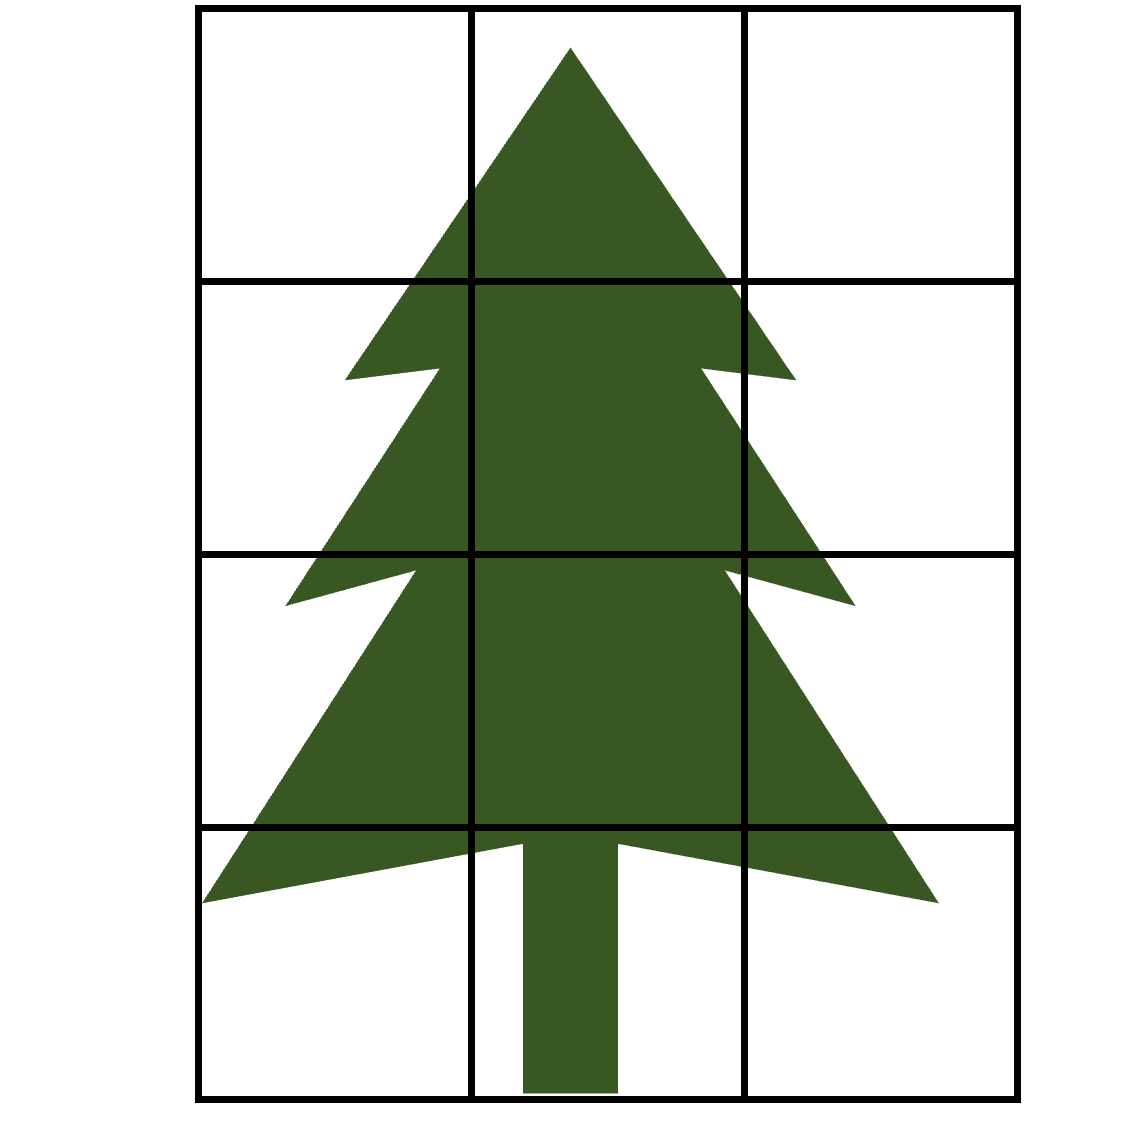
\includegraphics[height=4cm]{img/bounding_size_1.png}
        % \caption{}
        % \label{fig:bounding_size_1}
    \end{subfigure}
    \begin{subfigure}[b]{0.45\linewidth}
        \centering
        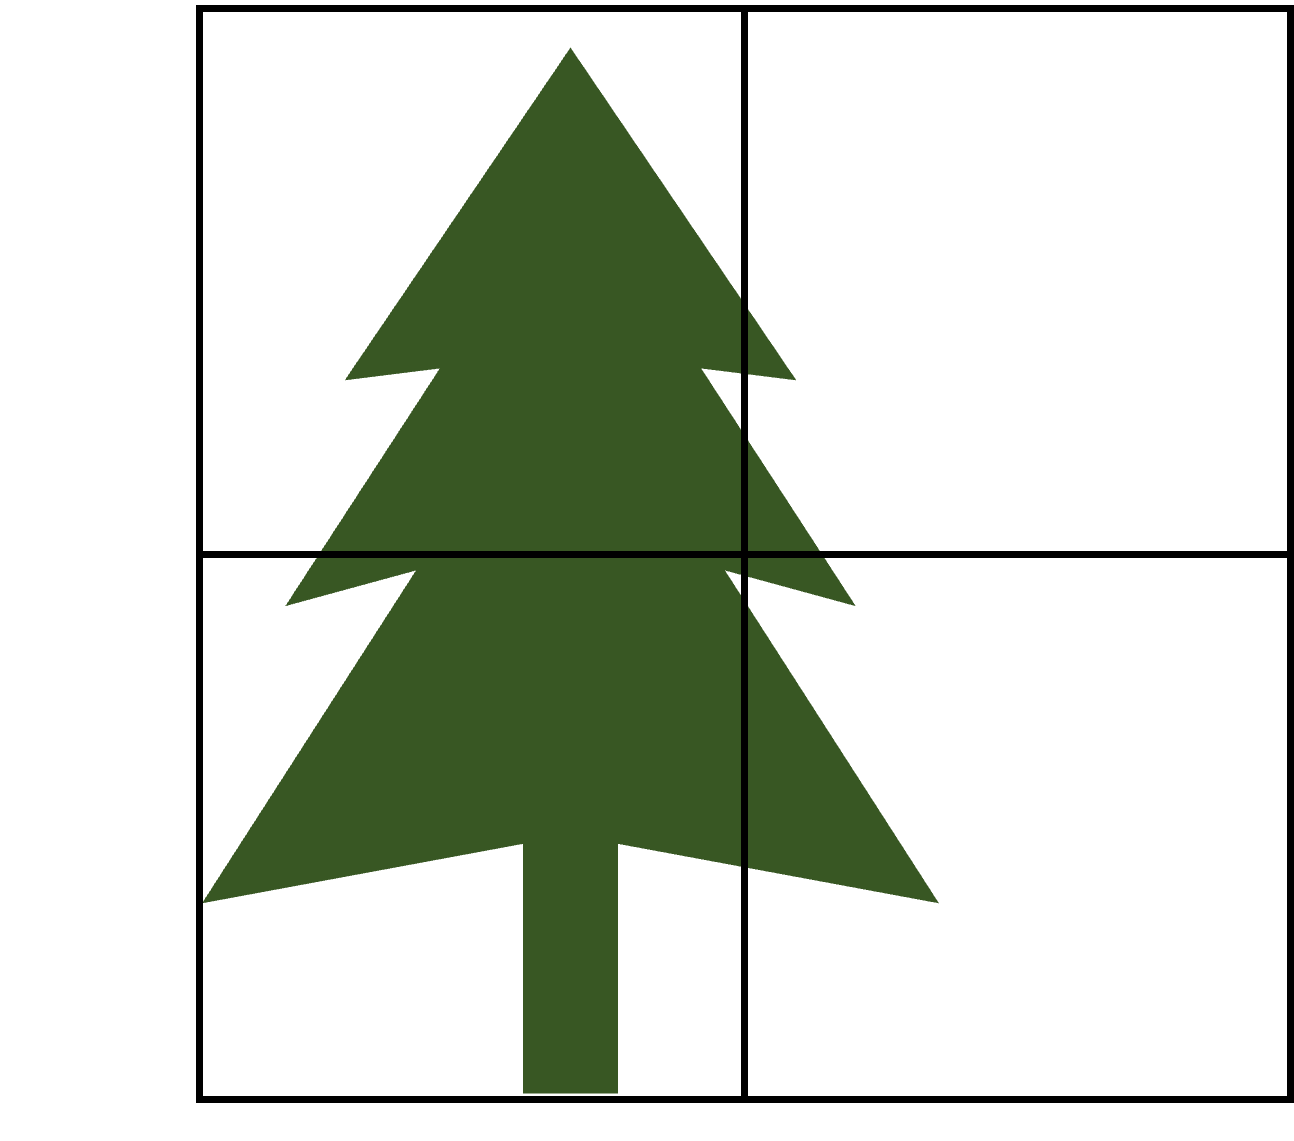
\includegraphics[height=4cm]{img/bounding_size_2.png}
        % \caption{}
        % \label{fig:bounding_size_2}
    \end{subfigure}
	\caption{The volume is always aligned to one side of the mesh. If we have different sized voxels (like \acsp{lod} necessarily have) the volume overlaps on one side and the bounding box sizes differ.}
	\label{fig:bounding_sizes}
\end{figure}
Then we sample a class \textit{Large}, \textit{Medium}, \textit{Small}, which contain tree models in the corresponding sizes.
This allows us to control the age of the forest, if we want an old forest we increase the probability for class \textit{Large} and if we want a rather young forest we increase the probability for \textit{Small} trees.
We then sample a tree in the chosen class and determine a position in the circle.
If we generate a scene with \acp{lod} we now have to determine the appropriate \ac{lod} for the model given the distance to the camera.
Knowledge of the camera position, gaze direction, the \ac{fov} and the sensor resolution are essential for that.
Note that a consequence is, that this information is baked into the scene description and moving the camera during rendering leads to a mismatch of the \acp{lod}.
Generating the scene in the renderer on the fly is currently no option, since this would lead to significantly worse performance of the renderer.
For positions outside the view frustum, we choose the coarsest \ac{lod} since these are not visible and only participate in indirect lighting.
If the position is inside the view frustum, we project the eight bounding box vertices of the coarsest volume on the image plane and compute the area of their convex hull using \texttt{scipy.spatial.ConvexHull}.
This gives us the number of pixels that the volume covers on the sensor.
We want to select \acp{lod} based on the heuristic that each voxel covers at most one pixel:
\begin{equation*}
    \frac{n_{voxel}}{n_{pixel}} > 1.
\end{equation*}
Therefore, we now have to compute the number of voxels that we see.
Calculating the product of the number of voxels in depth, height and width gives too many voxels, since some of the voxels are hidden by others.
Computing $depth \times height$, $depth \times width$ or $height \times width$ is only valid for viewing angles that are perpendicular to the surface of the voxel grid.
Another approach is to position a plane at the center of the grid and orient towards the camera.
The number of voxels that this plane intersects would then be a ground truth value for the voxels that we see.
Evaluating this however, is really expensive since each voxel has to be tested whether it intersects the plane.
We choose a faster approach that approximates this value and is depicted in Figure \ref{fig:voxel_estimation}.
\begin{figure}[ht]
    \centering
    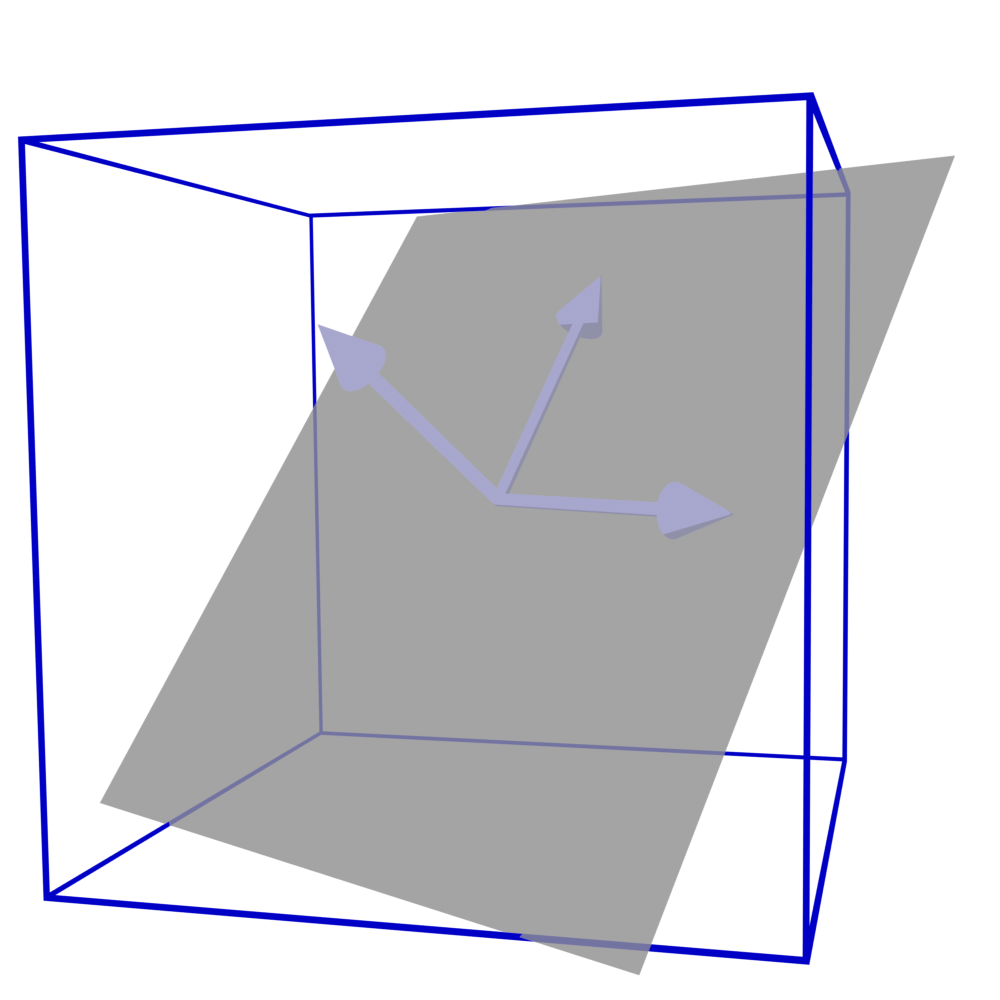
\includegraphics[width=0.3\linewidth]{img/voxel_estimation.png}
    % \includesvg[pretex=\tiny, width=1.0\linewidth]{img/pipeline}
    \caption{We estimate the number of intersected voxels by shooting two rays which are perpendicular to the camera direction (plane normal). After intersecting them with the bounding box we can construct a rectangle whose area approximates the number of voxels intersected by a plane. The true value is different, since a plane intersecting a cube can produce anything from a triangular to a hexagonal area.}
    \label{fig:voxel_estimation}
\end{figure}
From the center of the volume bounding box we shoot a ray perpendicular to the camera direction horizontally.
A second ray is shot in a direction perpendicular to the first ray and perpendicular to the direction towards the camera.
We intersect the rays with the bounding box which gives us the number of voxels they passed.
By multiplying the results from both rays we get the number of voxels a rectangle located at the bounding box center intersects.
The ground truth value for the number of intersected voxels by a plane can be different, since a plane intersecting a cube does not necessarily give a rectangle.
However we found that our approach closely approximates the true value.
Having computed the number of voxels we can now choose the coarsest \ac{lod} that still fulfills our heuristic.



\section{Rendering}
\label{sec:rendering}
We render meshes and volumes using path tracing.
Like our filtering implementation, our path-tracer is also \ac{gpu} accelerated using OptiX \cite{parker_optix}.
For fast convergence we employ next event estimation and use importance sampling of the scattering functions and the environment map.
Russian roulette is used to terminate insignificant paths.
In order to render scenes with many meshes and volumes, we use instancing.
A certain mesh or volume thus has to occupy \ac{gpu} memory just once and for each usage an instance is created, each with its own model transformation.

Our surfaces use the lambertian diffuse \cite{lambert} and the Trowbridge-Reitz \cite{trowbridge_reitz} microfacet \ac{brdf}, which is the general form of the GGX \ac{brdf}.
As Figure \ref{fig:leaf_gloss} shows, real leafs have a specular gloss, therefore we incorporate a specular \ac{brdf}.
\begin{figure}[ht]
    \centering
    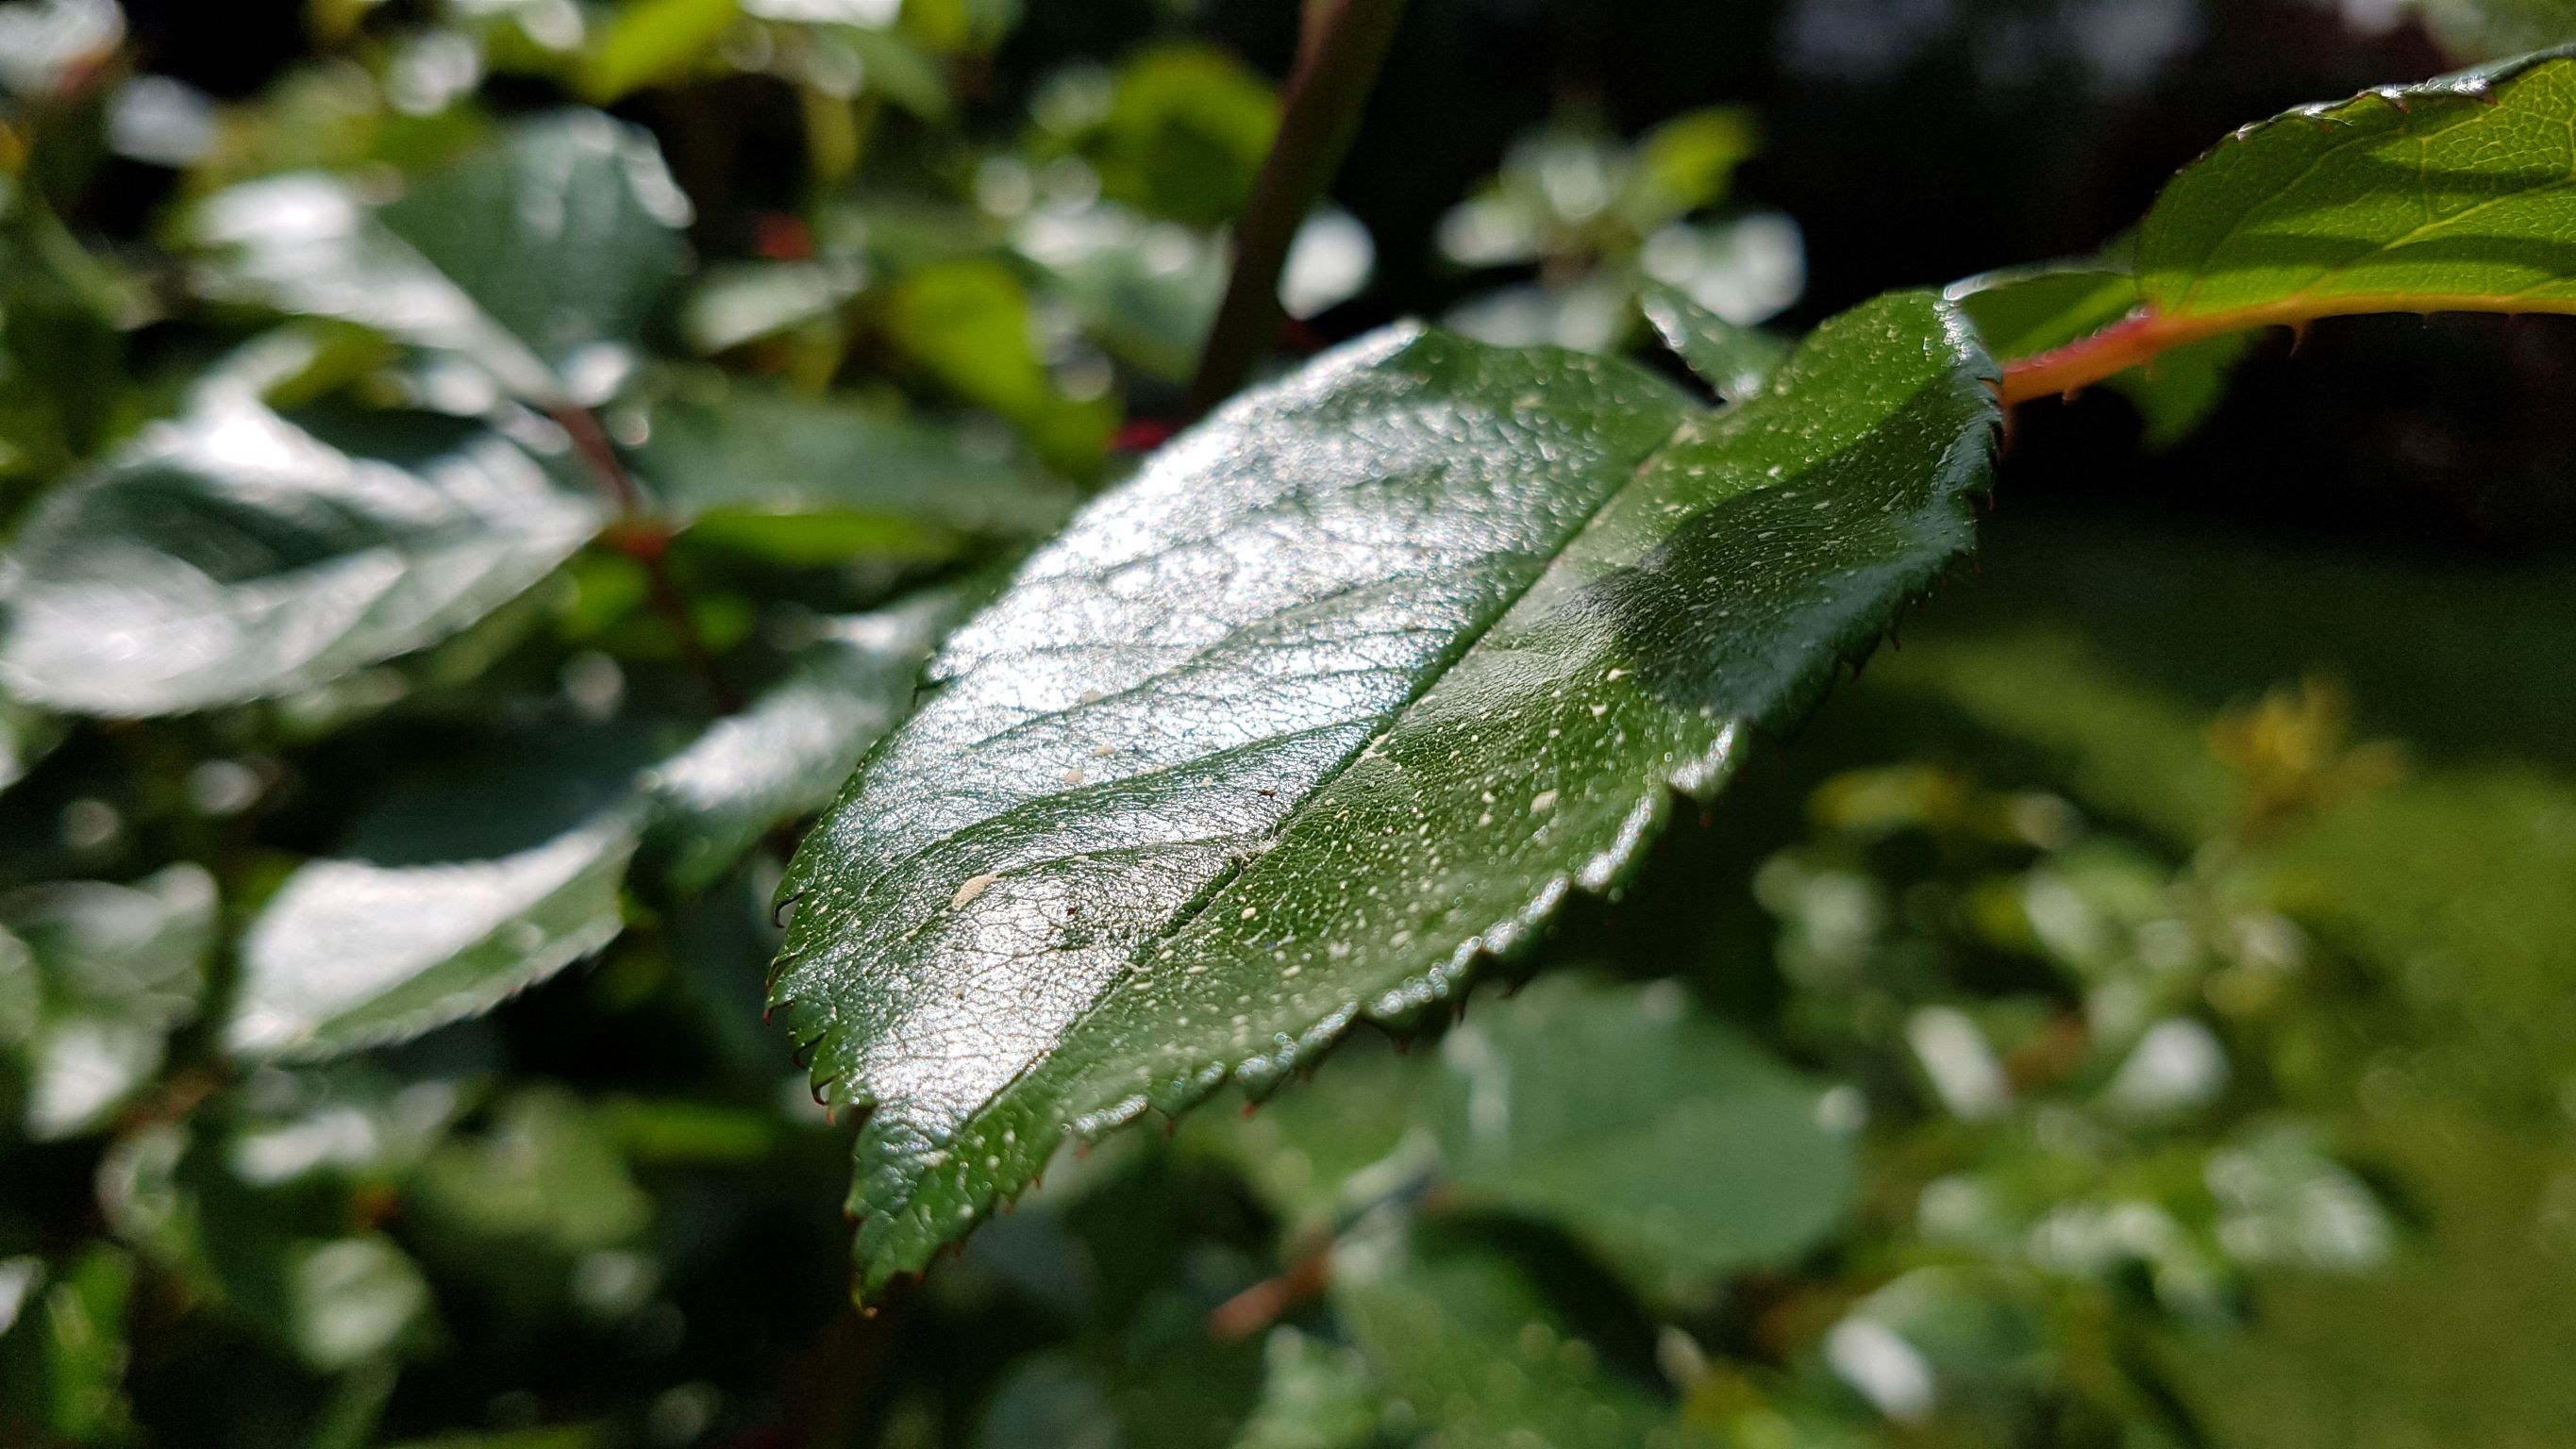
\includegraphics[width=0.5\linewidth]{img/leaf_gloss.jpg}
    % \includesvg[pretex=\tiny, width=1.0\linewidth]{img/pipeline}
    \caption{Real leafs often have a specular reflecting layer, therefore we incorporate a specular \ac{brdf} in our lighting calculations.}
    \label{fig:leaf_gloss}
\end{figure} 
The models we use neither have specular maps nor do they have a sensible specular color.
Therefore we compute the luminosity of the diffuse texture and use it as a specular map.
Figure \ref{fig:leaf_renderings} shows renderings of our approach of using the diffuse texture as a basis for the specular map.
\begin{figure}[ht]
    \centering
    \begin{subfigure}[b]{0.3\linewidth}
        \centering
        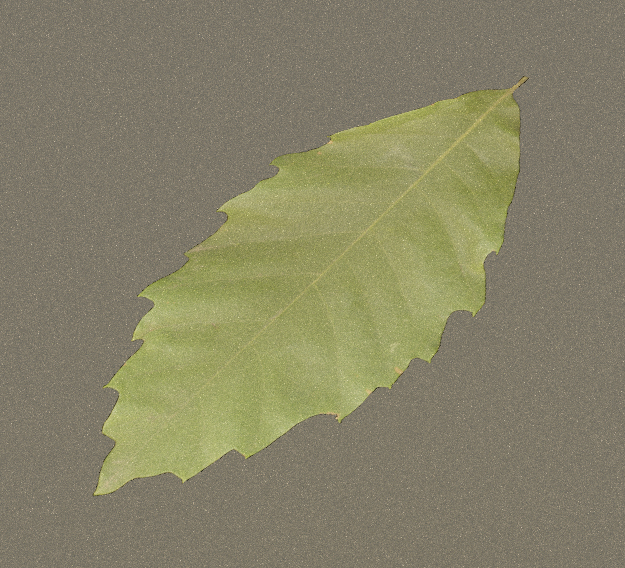
\includegraphics[width=1\linewidth]{img/leaf_no_spec.jpg}
        \caption{}
        % \label{fig:bounding_size_1}
    \end{subfigure}
    \begin{subfigure}[b]{0.3\linewidth}
        \centering
        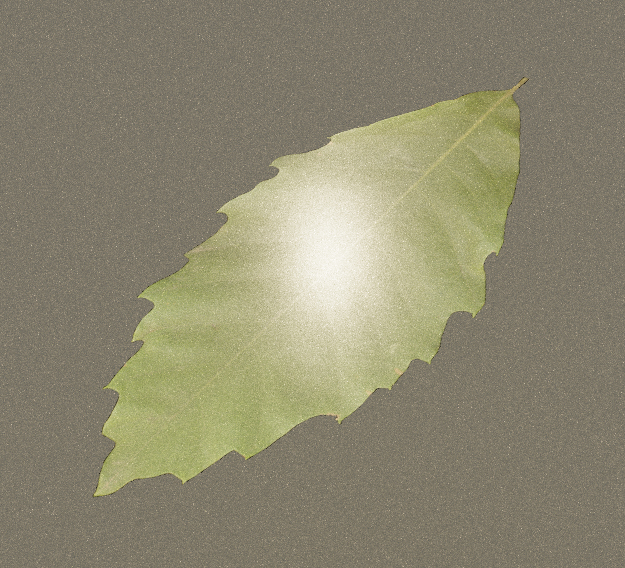
\includegraphics[width=1\linewidth]{img/leaf_spec.jpg}
        \caption{}
        % \label{fig:bounding_size_2}
    \end{subfigure}
	\caption{Renderings of leafs using the default material (a) and our modification of converting the diffuse texture to a specular map (b).}
	\label{fig:leaf_renderings}
\end{figure}
We combine the diffuse and microfacet \ac{brdf} using the Fresnel term $F$ \cite{fresnel}, which describes the amount of light reflected on a surface.
It evaluates to values close to one for grazing angles and to one when light hits the surface perpendicularly \cite{pbr}.
For a layered surface the effect of the diffuse reflection is biggest near perpendicular angles while specular reflection mostly is visible near grazing angles \cite{pbr}.
We can therefore write our combined \ac{brdf} as:
\begin{equation*}
    f(x, \omega_i, \omega_o) = F(|n_x \cdot \omega_o|)f_{spec}(x, \omega_i, \omega_o) + (1 - F(|n_x \cdot \omega_o|))f_{diff}(x, \omega_i, \omega_o).
\end{equation*}

As described in Section \ref{subsec:solving_beer_lambert_law_in_heterogeneous_media}, we use brick grid by \citeauthor{brick_grid} \cite{brick_grid} to represent the density values of a volume.
The authors also provide an implementation of the distance sampling procedure they use \cite{brick_grid}, which we rougly follow.
The full distance sampling algorithm that we use can be found in Appendix ..., in summary we use the distance sampling by \cite{brick_grid} until we find an interaction. % TODO: Add Appendix
We then perform a lookup in the NanoVDB grid to retrieve a filtered normal, diffuse and specular color, the index of refraction and the \ac{sggx} matrix $S$.
Since our procedure returns the albedo at this point of the medium, we now have to compute which frequencies of the light are absorbed, which is given by the color.
Just as for our surface rendering we apply the Fresnel term to weight the diffuse and specular color.
Because the Fresnel term requires a surface normal, we now use the filtered normal that we also stored in the NanoVDB grid.
We weight the specular color by $F$ and the diffuse color by $1-F$ to obtain our albedo.

At each sampled interaction in the medium we sample a new ray direction using the \ac{sggx} phase function.
Again we use the Fresnel term, this time to get a probability whether we should sample the diffuse phase function or the specular phase function.
Both phase functions rely on sampling a microflake normal from the \ac{sggx} \acl{vndf}.
In contrast to \citeauthor{sggx} \cite{sggx}, we do not align this microflake normal with the ray direction $\omega_o$, but with the filtered normal $n$.
Figure \ref{fig:tree_normal_maps} illustrates the normals of the mesh and when the microflake normal is aligned with direction $\omega_o$ or the filtered normal.
\begin{figure}[ht]
    \centering
    \begin{subfigure}[b]{0.3\linewidth}
        \centering
        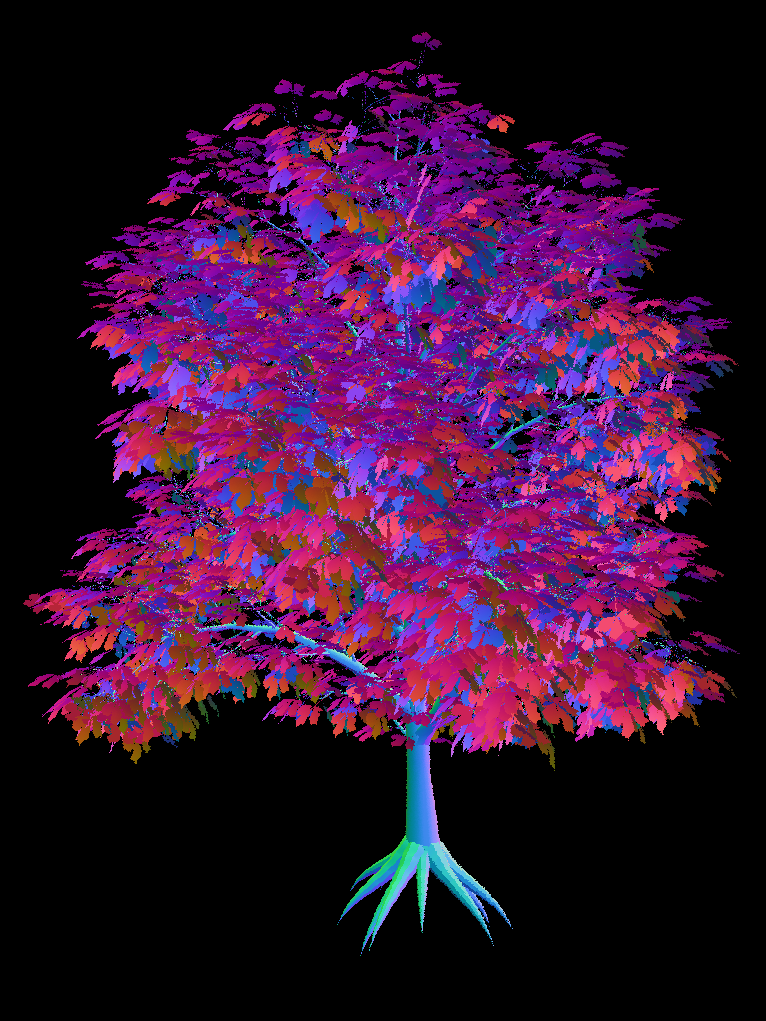
\includegraphics[width=1\linewidth]{img/normal_map_mesh.png}
        \caption{}
        % \label{fig:bounding_size_1}
    \end{subfigure}
    \begin{subfigure}[b]{0.3\linewidth}
        \centering
        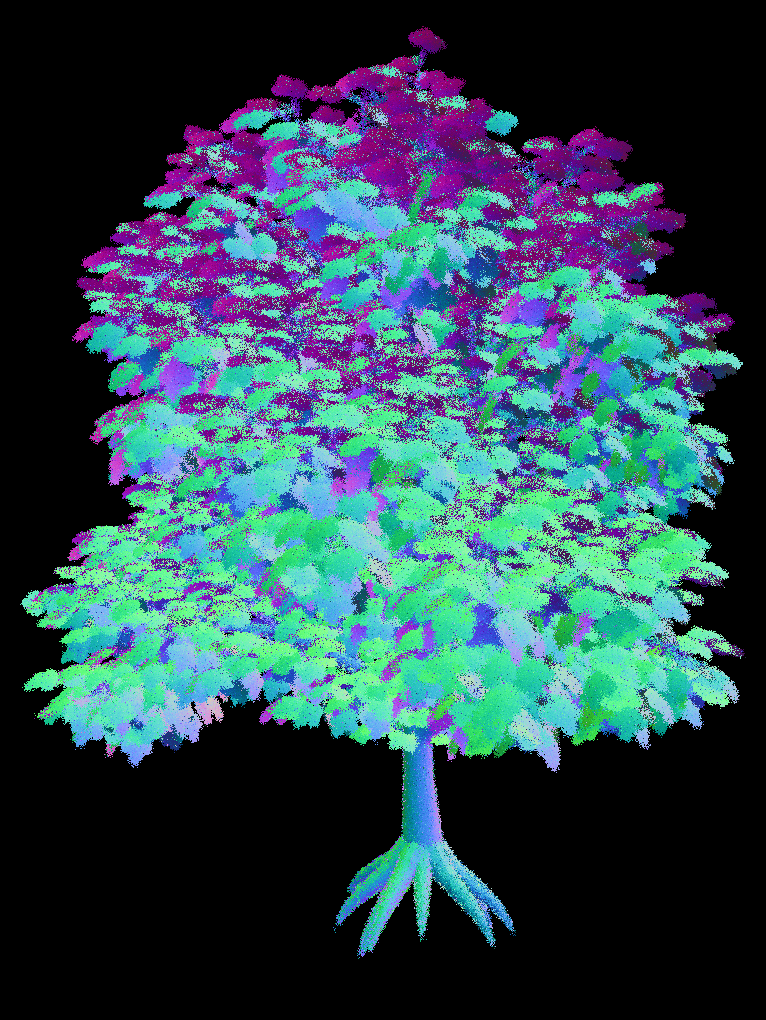
\includegraphics[width=1\linewidth]{img/normal_map_vndf_wo_aligned.png}
        \caption{}
        % \label{fig:bounding_size_2}
    \end{subfigure}
    \begin{subfigure}[b]{0.3\linewidth}
        \centering
        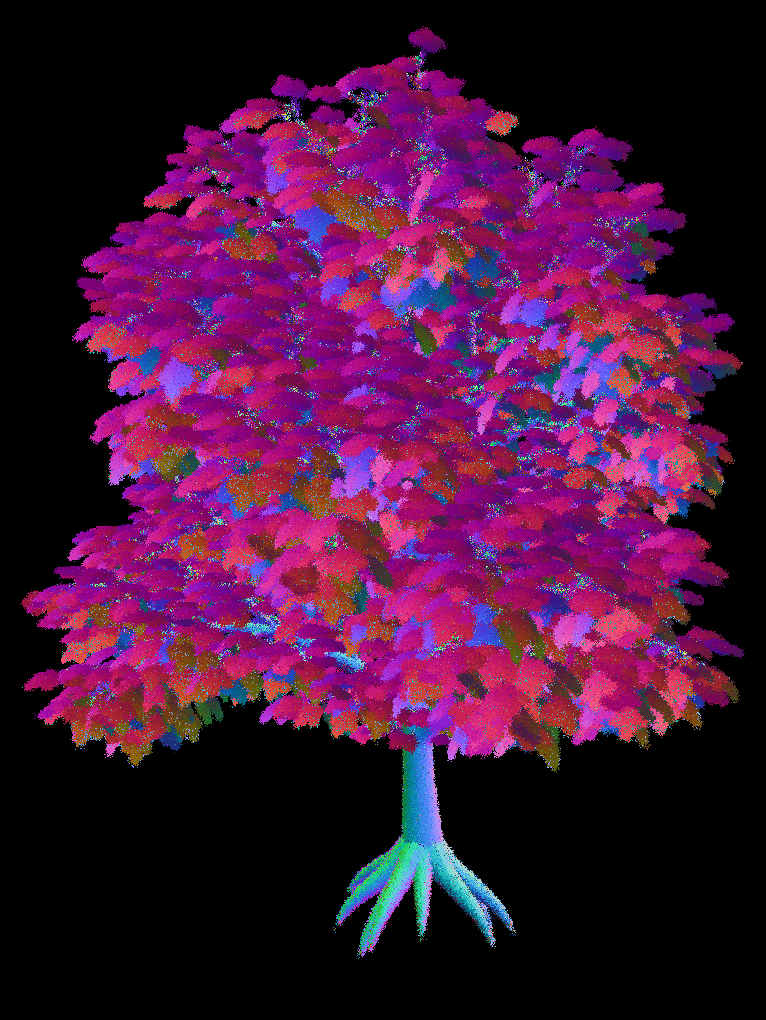
\includegraphics[width=1\linewidth]{img/normal_map_vndf_normal_aligned.png}
        \caption{}
        % \label{fig:bounding_size_1}
    \end{subfigure}
	\caption{Visualization of the normals of the surface mesh (a), and of volumetric \acsp{lod} when the microflake normal is aligned with the direction $\omega_o$ (b) and when it is aligned with the filtered normal (c) .}
	\label{fig:tree_normal_maps}
\end{figure}
It is obvious, that aligning the microflake normal with the outgoing direction $\omega_o$ gives different normals than the normals given by the mesh, while aligning it with the filtered normal gives normals that are distributed around the filtered normal.